%----------------------------------------------------------------------------------------
%
% LaTeX-template for degree projects at LNU, Department of Computer Science
% Last updated by Johan Hagelbäck, Mar 2017
% Linnaeus University
%
% License: Creative Commons BY
%
%----------------------------------------------------------------------------------------

%----------------------------------------------------------------------------------------
%	Settings and configuration
%----------------------------------------------------------------------------------------

\documentclass[a4paper,12pt]{article}

\renewcommand{\baselinestretch}{1}
\usepackage[dvipsnames]{xcolor}

\definecolor{green}{RGB}{0, 153, 0}
\definecolor{red}{RGB}{153, 0, 0}

\usepackage[utf8]{inputenc}
\usepackage{tabularx}
\usepackage{tikz}
\usepackage{minted}
\usetikzlibrary{arrows.meta, chains, fit}
\usepackage{lipsum}
\usepackage{listings}
\usepackage[T1]{fontenc}
\usepackage{times}
\usepackage[english]{babel}
\usepackage[utf8]{inputenc}
\usepackage{dtklogos}
\usepackage{wallpaper}
\usepackage[absolute]{textpos}
\usepackage{booktabs} 
\usepackage[top=2cm, bottom=2.5cm, left=3cm, right=3cm]{geometry}
\usepackage{appendix}
\usepackage[nottoc]{tocbibind}
\usepackage[colorlinks=true,
            linkcolor=black,
            urlcolor=blue,
            citecolor=black]{hyperref}
\usepackage{comment}
\setcounter{secnumdepth}{3}
\setcounter{tocdepth}{3}
\usepackage{graphicx}
\usepackage{amssymb} % for checkmarks
\usepackage{sectsty}
\sectionfont{\fontsize{14}{15}\selectfont}
\subsectionfont{\fontsize{12}{15}\selectfont}
\subsubsectionfont{\fontsize{12}{15}\selectfont}
\pagenumbering{arabic}
\setcounter{page}{1} % Specifies the starting page number

\usepackage{csquotes} % Used to handle citations

\renewcommand{\thetable}{\arabic{section}.\arabic{table}}  
\renewcommand{\thefigure}{\arabic{section}.\arabic{figure}} 

%----------------------------------------------------------------------------------------
%	
%----------------------------------------------------------------------------------------
\newsavebox{\mybox}
\newlength{\mydepth}
\newlength{\myheight}

\newenvironment{sidebar}%
{\begin{lrbox}{\mybox}\begin{minipage}{\textwidth}}%
{\end{minipage}\end{lrbox}%
 \settodepth{\mydepth}{\usebox{\mybox}}%
 \settoheight{\myheight}{\usebox{\mybox}}%
 \addtolength{\myheight}{\mydepth}%
 \noindent\makebox[0pt]{\hspace{-20pt}\rule[-\mydepth]{1pt}{\myheight}}%
 \usebox{\mybox}}

%----------------------------------------------------------------------------------------
%	Title section
%----------------------------------------------------------------------------------------
\newcommand\BackgroundPic{
    \put(-2,-3){
    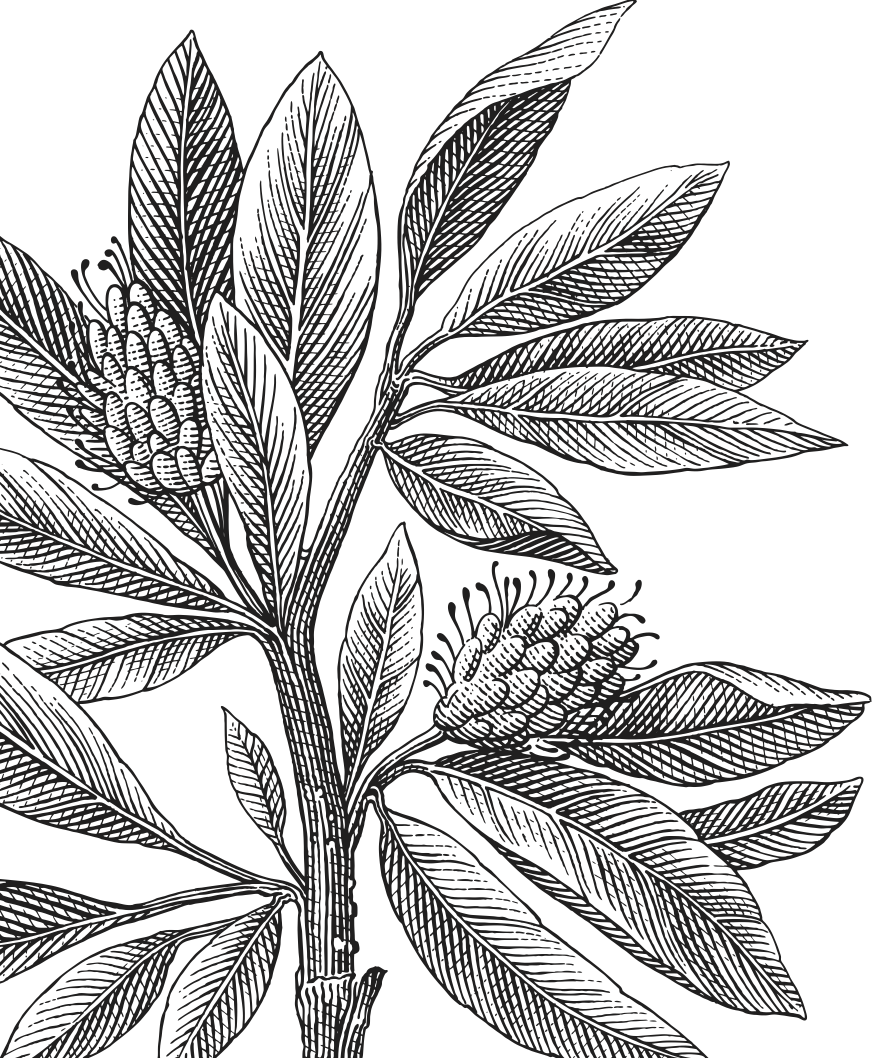
\includegraphics[keepaspectratio,scale=0.3]{img/lnu_etch.png} % Background picture
    }
}
\newcommand\BackgroundPicLogo{
    \put(30,690){
    
\includegraphics[keepaspectratio,scale=0.10]{img/logo.png} % Logo in upper left corner
    }
}

\title{	
\vspace{-8cm}
\begin{sidebar}
    \vspace{10cm}
    \normalfont \normalsize
    \Huge Bachelor Degree Project \\
    \vspace{-1.3cm}
\end{sidebar}
\vspace{3cm}
\begin{flushleft}
    \huge Reasoning models compared with traditional text classification methods \\ \large Exploring the efficiency and accuracy of labeling multi-level categories and subcategory structure
\end{flushleft}
\null
\vfill
% \begin{textblock}{8}(8,13)
\begin{textblock}{8}(7.5,13)
\begin{flushright}
\begin{minipage}{\textwidth}
\begin{flushleft} \large
\emph{Authors:} Samuel Svensson \& Andreas Nilsson\\
\emph{Supervisor:} Daniel Toll\\
\emph{Examiner:} Amilcar Soares Junior\\
\emph{Semester:} VT25\\
\emph{Subject:} Computer Science\\
\end{flushleft}
\end{minipage}
\end{flushright}
\end{textblock}
}

\date{} 

\begin{document}
\pagenumbering{gobble}
\newgeometry{left=5cm}

\textbf{\large{Preface}}\\

\noindent 
We would like to express our gratitude to several individuals who played important roles in assisting us in completing this thesis. Firstly, ...... 

%----------------------------------------------------------------------------------------
\newpage
\pagenumbering{gobble}
\AddToShipoutPicture*{\BackgroundPic}
\AddToShipoutPicture*{\BackgroundPicLogo}
\maketitle
\restoregeometry
\clearpage
\tableofcontents
\newpage

\section{Introduction}

This paper introduces the different aspects of the research and to provide the
main scope.
It will describe large language models (LLMs) and their applications in text
classification.
We will collaborate with UPTILT that delivers an application to customers within
the service business, solving the delivery of invoices and offers to the
customer by tracking materials, hourly work and more.
They have provided us with the necessary data which has been redacted to ensure
anonymity and privacy.
We will foremost discuss the importance of classifying work orders (WOs), but
also provide a general conclusion on the topic and contribute to the field of
text classification and natural language processing (NLP) using LLMs.

\subsection{Background}

In many industries today, working with and handling large quantities of
structured and unstructured data is extremely important.
One example is text classification which labels text based on their content.
Traditionally, machine learning (ML) methods have been used for this purpose,
but recently, LLMs have shown potential posing generative capabilities, along
with understanding and reasoning within language(s)
\cite{huang2024} \cite{zhang2024}.

Training a ML model means analyzing the content of the text and identifying
features that are relevant, so computer systems can, for example, use this
technique for identifying spam and filtering documents \cite{dalal2011}.
Comparing this approach to an already widely trained LLM model, which does not
require the same amount of manual labor and configuration.

LLMs are a subgroup of AI that work on the knowledge of next word context and
are often utilized in the context of allowing the user to prompt it with
instructions or questions.
They utilizes a much larger pre-trained knowledge compared to machine learning,
which often specializes in a specific domain and type of data.
Furthermore, they can analyze data and recognize patterns with minimal human
interaction, and makes them highly effective in applications like NLP
\cite{andersson2024}.

WOs is a document that outlines the details of a maintenance task.
This data comes in the form of text and can through proper utilization be the
key component when categorizing using LLMs.
WOs most commonly contains information regarding the material required to
complete such task, but also the geographic location, customer etc.
Today, many companies still rely on manual processing, which often leads to
mistakes \cite{ibm2023} \cite{li2024}.
Throughout our work, we will focus on providing a better solution than the
current manual processing by using LLMs to classify work orders.

\subsubsection{Related Work}

Huang and He \cite{huang2024} explain the cost of manual labor when it comes to
tagging and categorizing text.
Furthermore, the fine-tuning and choice of parameters can influence the final
behavior of the trained ML model.
They explain how the latest LLMs have showcased "remarkable reasoning
performance across a wide range of NLP tasks".
We aim to follow this trail and further analyze the efficiency and performance
of categorizing text within the context of WOs.

\bigskip
Recent advances in LLMs have shown that they can be fine-tuned to effectively
classify structured data.
For example, GPT-4, LLaMA 2, and ChatGLM 2 have shown remarkable performance in
text classification \cite{zhang2024}.
We will be discussing and evaluating the efficiency and accuracy of using LLMs
to classify structured WOs, unlike previous studies, which focuses more on
general NLP tasks.
Our paper gives an insight into whether they can be used with correct prompting
to classify WOs.

\bigskip
Current research has demonstrated that transformer-based models
(a neural network architecture, meaning it learns by tracking relationships
between words \cite{merritt2022}),
such as BERT and other domain-specific variants, significantly improve text
classification processes through transfer learning and fine-tuning
\cite{nazyrova2024}.
While Nazyrova et al. focuses on medical text classification and our focus lies
within WO classification, their findings on the topic of fine-tuning LLMs is
relevant for our paper and its research.

\section{Theoretical Background}

Data typically fall into two primary categories: structured and unstructured. Structured data are characterized by a well-defined, predefined format, often organized in tables where rows represent entities and columns represent specific attributes. Examples include relational databases, spreadsheets containing employee records with distinct fields (ID, name, department), or financial reports with clearly defined columns for dates, categories, and values. This inherent organization makes structured data readily amenable to querying and analysis using standard tools.

In contrast, unstructured data lack a predefined data model or organizational schema. This category represents a large majority of the data generated today and includes diverse sources such as emails, text documents, social media content, images, videos, and operational logs such as Work Orders (WOs) relevant to this study. A typical WO, for instance, may contain free-form text describing maintenance procedures, lists of materials, location information, and customer details, none of which conform to a rigid structure \cite{ibm2023work}. Due to this variability and lack of explicit organization, unstructured data cannot be easily stored or analyzed using traditional tabular methods and presents unique challenges \cite{ibm2025datadiff}.

Despite the analytical challenges, unstructured text data often contains substantial valuable information. The significant volume and complexity of this data requires the use of automated techniques to process, categorize, and extract meaningful insights. Within the field of Natural Language Processing (NLP), text classification stands out as a fundamental method developed precisely for this purpose. It is the task of automatically assigning predefined labels or categories to text documents based on their content. Applying text classification to resources like WOs, emails, or reports helps impose a useful structure, enabling better organization and downstream analysis.

Historically, the task of text classification has been approached using various machine learning (ML) methodologies. Early techniques often involved rule-based systems or classical supervised algorithms such as Logistic Regression and Naive Bayes. A critical prerequisite for applying these traditional algorithms to text was feature engineering. Since these models typically require numerical input, feature engineering involved processes to identify and extract relevant textual characteristics (e.g., word frequencies via Term Frequency-Inverse Document Frequency (TF-IDF), presence of specific n-grams, Bag-of-Words representations) and convert them into a structured vector format suitable for the ML model \cite{bing2011mining}.


However, the early techniques often fall short in capturing language nuances, context details, and the ambiguity in unstructured text. More recently, advances in natural language processing (NLP) have led to the development of large language models (LLMs) based on transformer architectures such as GPT and BERT. These models use self-attention to focus on important parts of the text and capture deep meaning by understanding relationships between words. There are even newer versions that add reasoning capabilities, which aim to improve decision-making in text classification. Learning from vast amounts of pre-trained data and use self-attention to track relationships between words, which significantly improves their ability to understand and predict next word context. For example, while traditional ML models focus on manually extracting features, modern LLMs such as the previously mentioned GPT and BERT can adapt to various types of text with minimal human intervention such as pre processing and structuring. Supporting this development, recent research has shown that LLMs -- especially when fine-tuned for particular domains -- exhibit not only advanced language understanding but also reasoning capabilities that can further improve text classification performance \cite{huang2024classification, andersson2024ikea, merritt2022transformer, nazyrova2024medical, wang2024classifiers}, capabilities central to the comparisons explored in this work (RQ1, RQ2, RQ3).

One of the most significant advantages of large language models over traditional approaches is their ability to generalize to new tasks using \textbf{zero-shot}, \textbf{one-shot}, and \textbf{few-shot} learning \cite{brown2020language}. These concepts refer to how much prior labeled data a model needs to perform a task. Zero-shot learning allows an LLM to classify text without being explicitly trained on any labeled examples. The model uses pre-trained knowledge to infer the most likely category based on a prompt describing the task. One-shot learning improves upon this by giving the model just one labeled example before making the classification. Finally, few-shot learning further enhances accuracy by providing multiple labeled examples in the prompt, allowing the model to generalize more effectively without requiring full retraining.

Switching focus to a machine learning technique such as recurrent neural networks or long short-term memory (LSTMs) shows capability in handling sequences of words and remembering long distances between related words. This makes it easier for the model to understand context without needing manual feature design. This technique was introduced in the late 90's and is far less complex and resource consuming than the latter transformer technique and is still considered a state-of-the-art algorithm \cite{wang2024classifiers, hochreiter1997long}. However, training and testing an RNN och LSTM model still requires a significant amount of resources when using a large dataset.

These datasets often require some processing involving actions such as bag of words (BoW) and term frequency-inverse document frequency (TF-IDF). Briefly explained, \cite{murel2024bagofwords} bag of words involves collecting the frequency of words in documents; more specifically, it's a feature extraction technique that models text data by creating an unstructured collection of all words in a document. The collection solely represents how often the words appear while ignoring grammar, word order, and context. Building upon this concept is TF-IDF, which can be described as a variation that further accounts for word frequency not just within one document, but across a whole corpus (a large collection of writings of a specific kind or on a specific subject), effectively giving more weight to terms that are significant to a specific document compared to common words found everywhere.

Although as Nazyrova et al. \cite{nazyrova2024medical} focuses on the medical application area within text classification, the principles are directly applicable to our context. Traditionally, companies rely on manual processing of WOs, a practice that is both labor-intensive and error prone \cite{li2024work}.



\section{Method}
% https://www.scribbr.com/dissertation/methodology/
%
% It should include:
%
% The type of research you conducted
% How you collected and analyzed your data
% Any tools or materials you used in the research
% How you mitigated or avoided research biases
% Why you chose these methods
%
% Your methodology section should generally be written in the PAST TENSE!

% --------------------------------------------
\subsection{Experiment design}
% Step 1:
% Methodological approach
%
% Research problem:
% Gain more understanding
%
% Type of data?
%
% How data was collected?
% Primary (collect by myself) or Secondary (collected by someone else) data:
We conducted a quantitative experimental study to evaluate the performance of two
models, Deepseek and Deepseek (reasoning), on the UPTILT dataset. Metrics such
as accuracy, precision, recall, F1 score, and execution time were collected
using primary data obtained through controlled experiments. This approach was chosen
to ensure measurable and reproducible results.

\subsubsection{Independent variables}
% Not sure if this is correct outlining the variables like this but may be useful
% to get the general idea of what we are working with:
\begin{center}
    \begin{tabular}{| l | l |}
        Dataset & The UPTILT dataset used for training and evaluation.     \\
        Models  & The different models used (both LLMs and ML algorithms). \\
    \end{tabular}
\end{center}

\subsubsection{Dependent variables}

\begin{center}
    \begin{tabular}{| l | l |}
        Accuracy            & The overall correctness of the model.           \\
        Precision           & The correctness of positive predictions.        \\
        Recall              & The ability to identify all relevant instances. \\
        F1 score            & A combined metric of precision and recall.      \\
        Execution time (ms) & The computational efficiency of each model.     \\
    \end{tabular}
\end{center}

% --------------------------------------------
\subsection{Data Collection}
% Step 2:
% Methods of data collection
%
% The sampling method or critera
% The tools, procedures, and materials
% How variables were measured
%
% Explain the table structure here as well!
% See Oxana's model/image in Slack.
\textcolor{blue}{Explain the tools and methods used to collect the data for our
result. Furthermore, explain the variables that were measured. See comments...}

\subsubsection{Models}
% Specify the LLMs and ML models/algorithms used (e.g., GPT-4o, Deepseek, Naive Bayes).
%
% Explain why these models were chosen and how they are relevant to the research question.

\subsubsection{Configurations}
% Describe whether the models are pre-trained, fine-tuned, or used with prompt engineering.
% Explain any hyperparameter tuning performed (e.g., learning rate, batch size).
% Discuss the computational resources required (e.g., GPUs, cloud services).
%
% Use references to support our choices here!

% --------------------------------------------
\subsection{Data Analysis}
% Step 3:
% Describe the methods of analysis
% (i.e. how you processed and analyzed the data).
%
% Quantitative data:
% Data preparation
% Software
% Statistical methods
%
% Analysis based of:
% Language
% Images
% Interpretations
% Themes and Patterns
\textcolor{blue}{Explain the methods used to analyze the collected data. See comments...}

% --------------------------------------------
\subsection{Research Biases}
% Step 4:
% Evaluate and justify methodological choices
%
% Why you chose these particular methods
% Why other methods were not suitable for your objectives
% How this approach contributes new knowledge or understanding
\section{Implementation}
\section{Results}
\subsection{Result 1...}
\subsection{Data analysis}
% Step 3:
% Describe the methods of analysis (how you processed and analyzed the data)
%
% A rigorous skepticism should be a part of every experiment:
% - Is this really a correct (fair) comparison?
% - Can we really draw these conclusions based on this experiment?
% - Have we taken all independent variables into account?
% - Are the measurements correct?

\subsection{Research biases (reliability and validity)}
% Step 4:
% Evaluate and justify methodological choices
%
% Why you chose these particular methods?
% Why other methods were not suitable for your objectives?
% How this approach contributes new knowledge or understanding?

\section{Discussion}
\section{Conclusions and Future Work}
\newpage
\bibliographystyle{IEEEtran}
\bibliography{references}
\end{document}